
% \begin{wrapfigure}{r}{0.48\textwidth}
%   \vspace{-20pt}
%   \centering
%   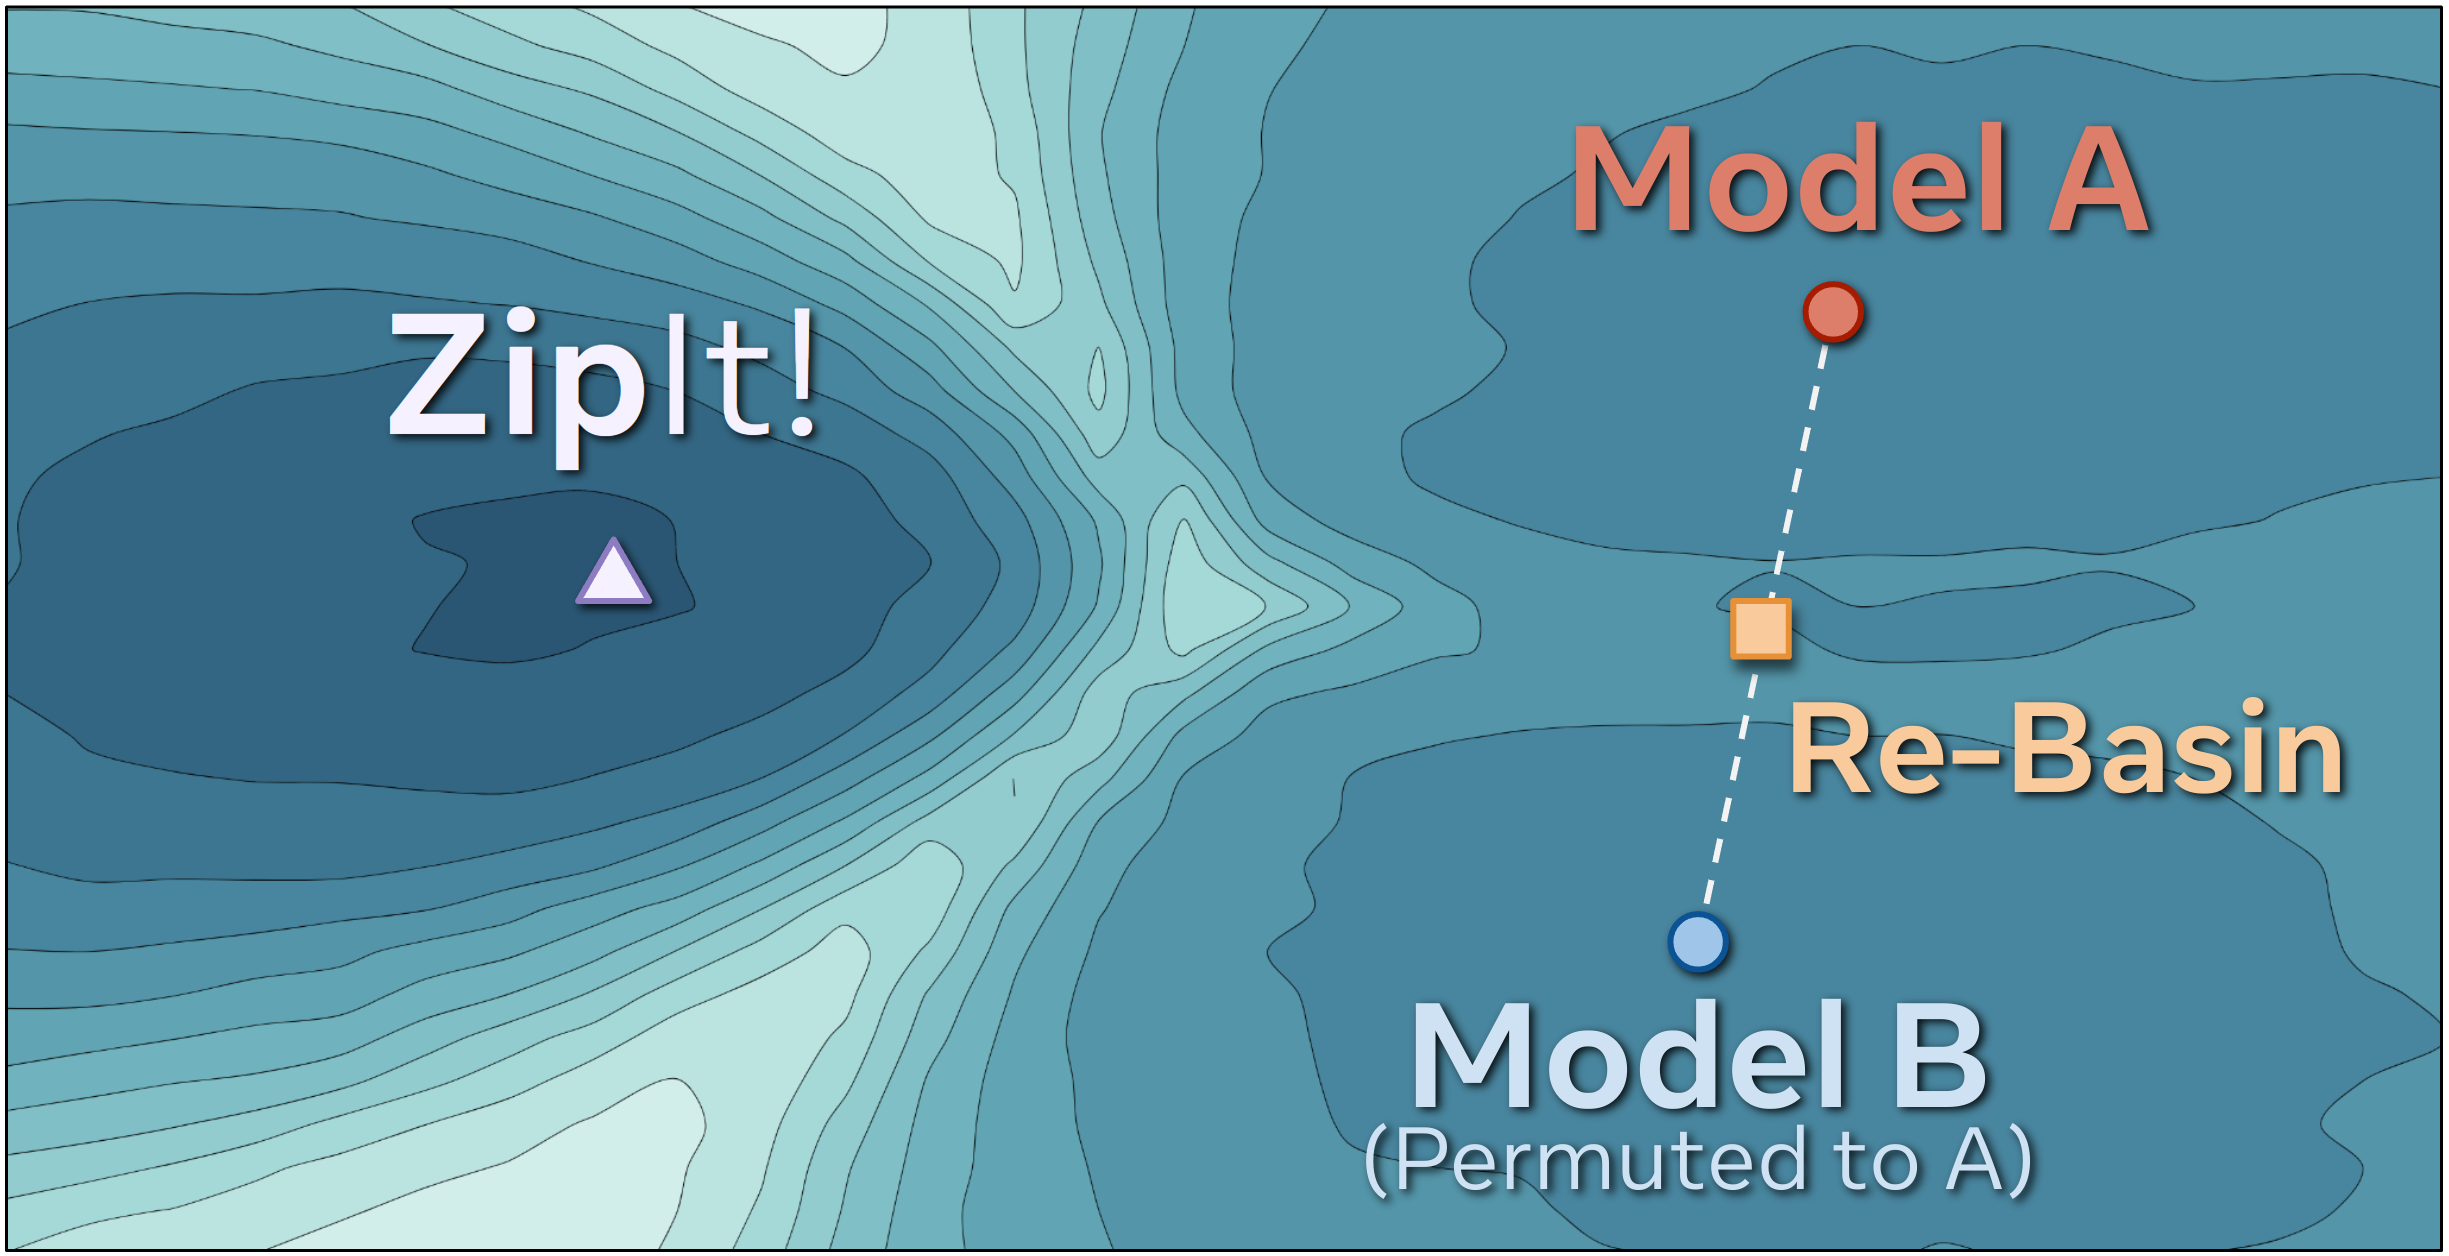
\includegraphics[width=\linewidth]{figures/imgs/loss_basin.png}
%   \newline
%   \caption{{\bf Prior Work Fails} on merging models trained on \textit{different} tasks. Git Re-Basin \cite{ainsworth2022git} assumes the two models lie in the same loss basin \textit{modulo permutation} and interpolates between them. However, that is not sufficient when the models are trained on \textit{different} tasks, here shown for disjoint class sets of CIFAR-100. While \modela{A} and the permuted \modelb{B} lie in similar basins, Git Re-Basin's interpolation performs \textit{worse} than the originals. In contrast, our method \name\ merges them into an even better model in a completely different loss basin.}
%   \label{fig:loss_basin}
%   \vspace{-50pt}
% \end{wrapfigure}



\begin{figure}
  \centering
  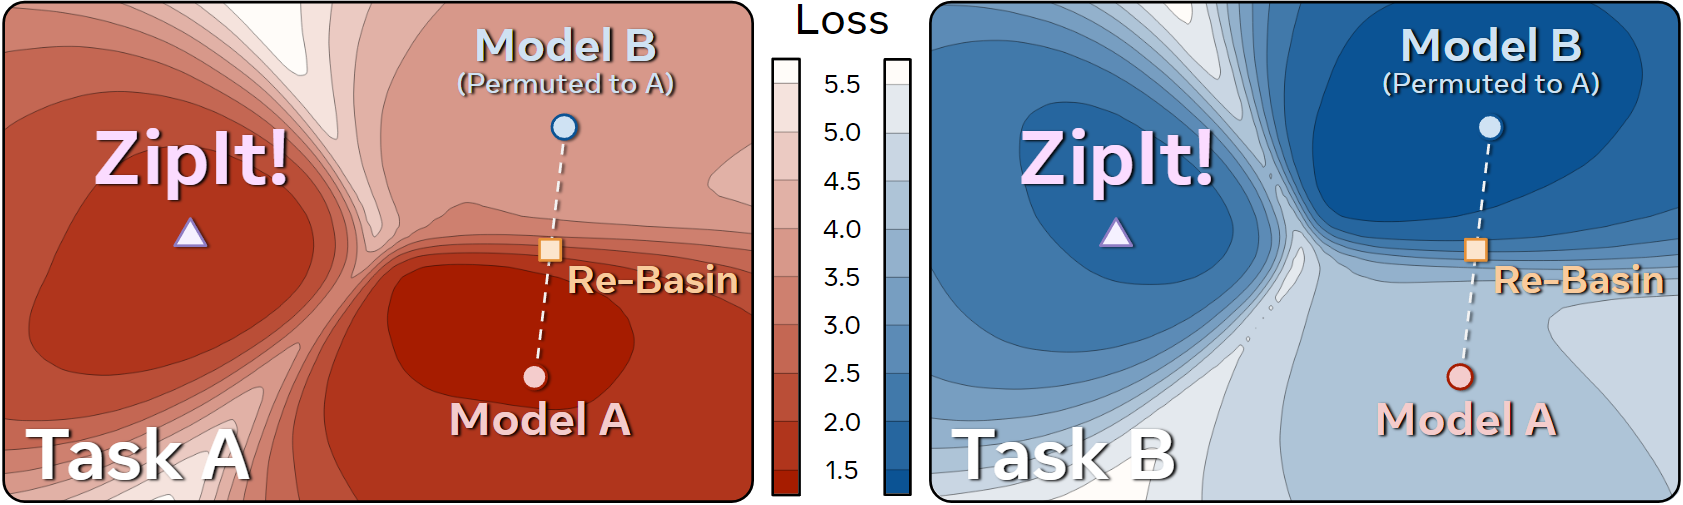
\includegraphics[width=\linewidth]{figures/imgs/loss_landscapes.png}
  % \newline
  % \vspace{-0.5em}
  \caption{{\bf Task Loss Landscapes} for models in Tab.~\ref{tab:cifar50+50}. % Prior work fails on merging models trained on different tasks: 
  \modela{Model A} and \modelb{Model B} lie in low loss basins for their own tasks, but \textit{not for the other task}.
  % While \modelb{Model B} lies in a low loss basin for \modelb{Task B}, it doesn't for \modela{Task A}, even after permuting it to \modela{Model A}.
  % because permuted models for \modela{Task A} likely \textit{do not} lie in a low loss basin for \modelb{Task B}.
  Thus, any interpolation between \modela{Model A} and a permuted \modelb{Model B} (e.g., Git Re-basin) lies outside the minima \textit{for both tasks} and thus performs poorly. In contrast, \name{}\ improves the merge by finding a model that lies in a low loss basin for both.
  % by finding a loss basin common to both tasks.
  % Git Re-Basin~\citet{ainsworth2022git} assumes the two models likely lie in the same loss basin \textit{modulo permutation} and interpolates between them. However, this is substantially less likely when the models are trained on \textit{different} tasks, here shown for disjoint class sets of CIFAR-100. While \modela{A} and \modelb{B} lie in basins on their respective tasks, these \textit{are not} shared across tasks. Thus, Git Re-Basin's interpolation performs \textit{worse} than the original's. In contrast, our method \name{}\ significantly improves the merge by finding a basin common to both tasks. 
  }
  \label{fig:loss_basin}
\end{figure}